% This example is meant to be compiled with lualatex or xelatex
% The theme itself also supports pdflatex
\PassOptionsToPackage{unicode}{hyperref}
\documentclass[aspectratio=1610, 9pt]{beamer}

% Load packages you need here
\usepackage[american]{babel}

\usepackage[autostyle]{csquotes}


\usepackage{amsmath}
\usepackage{amssymb}
\usepackage{mathtools}
\usepackage{xfrac}

\usepackage{tikz}
\usetikzlibrary{arrows.meta}
\usepackage[
  separate-uncertainty=true,
  per-mode=symbol-or-fraction,
]{siunitx}

\usepackage{fontawesome5}

% nice tables
\usepackage{tabularray}
\usepackage[outputdir=build]{minted}
\usemintedstyle{solarized-dark}

% colors
\usepackage{xcolor}
\definecolor{lightblue}{RGB}{0, 152, 195}
\definecolor{darkblue}{RGB}{6, 17, 45}
\definecolor{apps}{RGB}{136, 181, 91}

\usepackage{hyperref}
\usepackage{bookmark}

% load the theme after all packages

\usetheme[dark]{tudo}

% Put settings here, like
\unimathsetup{
  math-style=ISO,
  bold-style=ISO,
  nabla=upright,
  partial=upright,
  mathrm=sym,
}

\title{ctapipe -- Prototype Open Event Reconstruction Pipeline for the Cherenkov Telescope Array}
\author[M.~Linhoff]{\emph{Maximilian Linhoff}, Lukas Nickel, Noah Biederbeck for the CTA Consortium and Observatory}
\institute[{%
  \begin{tikzpicture}[baseline=(node.south)]
    \node[text width=5cm, align=right] (node) at (0, 0) {Astroparticle Physics\\WG Rhode \& Elsässer};
  \end{tikzpicture}
}]{Supported by the DFG (SFB 876 \& 1491) and the BMBF (ErUM Pro CTA-D)}
\titlegraphic{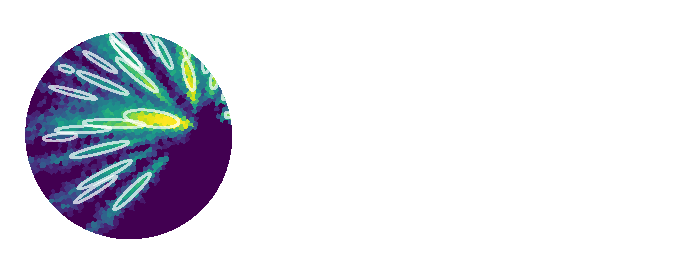
\includegraphics[height=0.4\textheight]{ctapipe-logo-dark.pdf}}
\date{2023-03-22}


\begin{document}

\maketitle

\begin{frame}{The Cherenkov Telescope Array Observatory}
  \begin{columns}[onlytextwidth, c]%
    \begin{column}{0.75\textwidth}%
      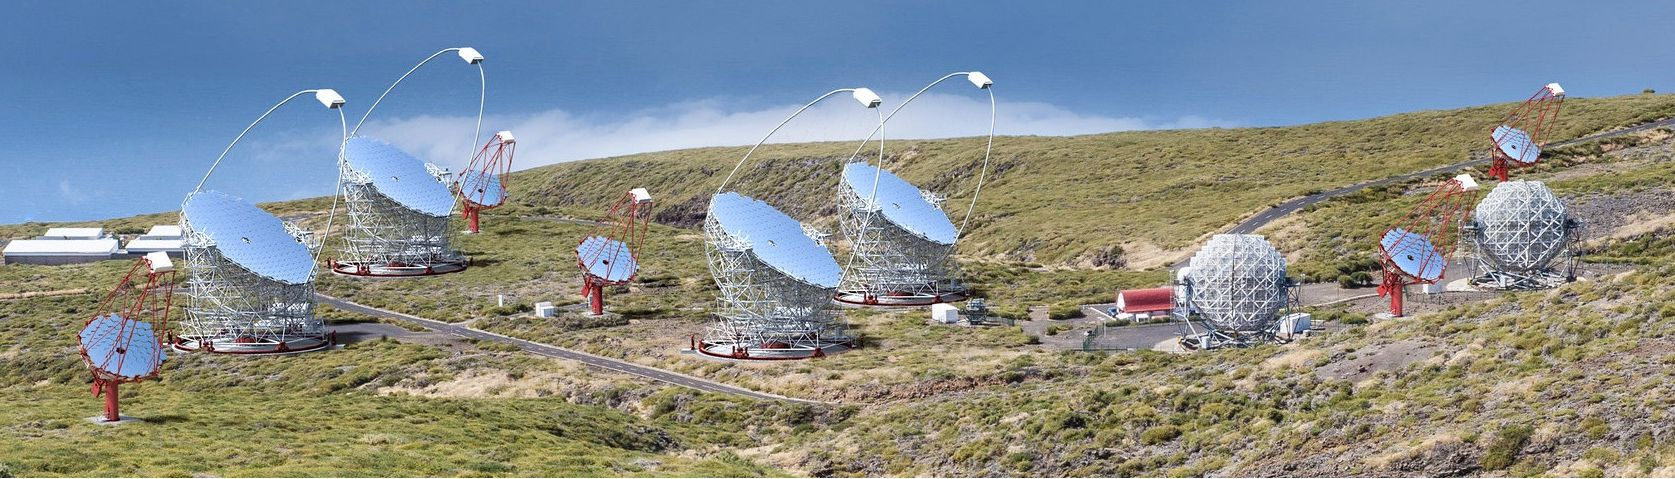
\includegraphics[width=\linewidth]{images/cta_north.jpg}
    \end{column}%
    \hfill%
    \begin{column}{0.24\textwidth}%
      CTA North (ORM, La Palma) \\
      4 LSTs, 9 MSTs (Alpha)\\
      LST-1 observing since 2018
    \end{column}%
  \end{columns}
  \medskip
  \begin{columns}[onlytextwidth, c]%
    \begin{column}{0.24\textwidth}%
      CTA South (ORM, La Palma) \\
      14 MSTs, 37 SSTs  (Alpha)\\
    \end{column}%
    \hfill%
    \begin{column}{0.74\textwidth}%
      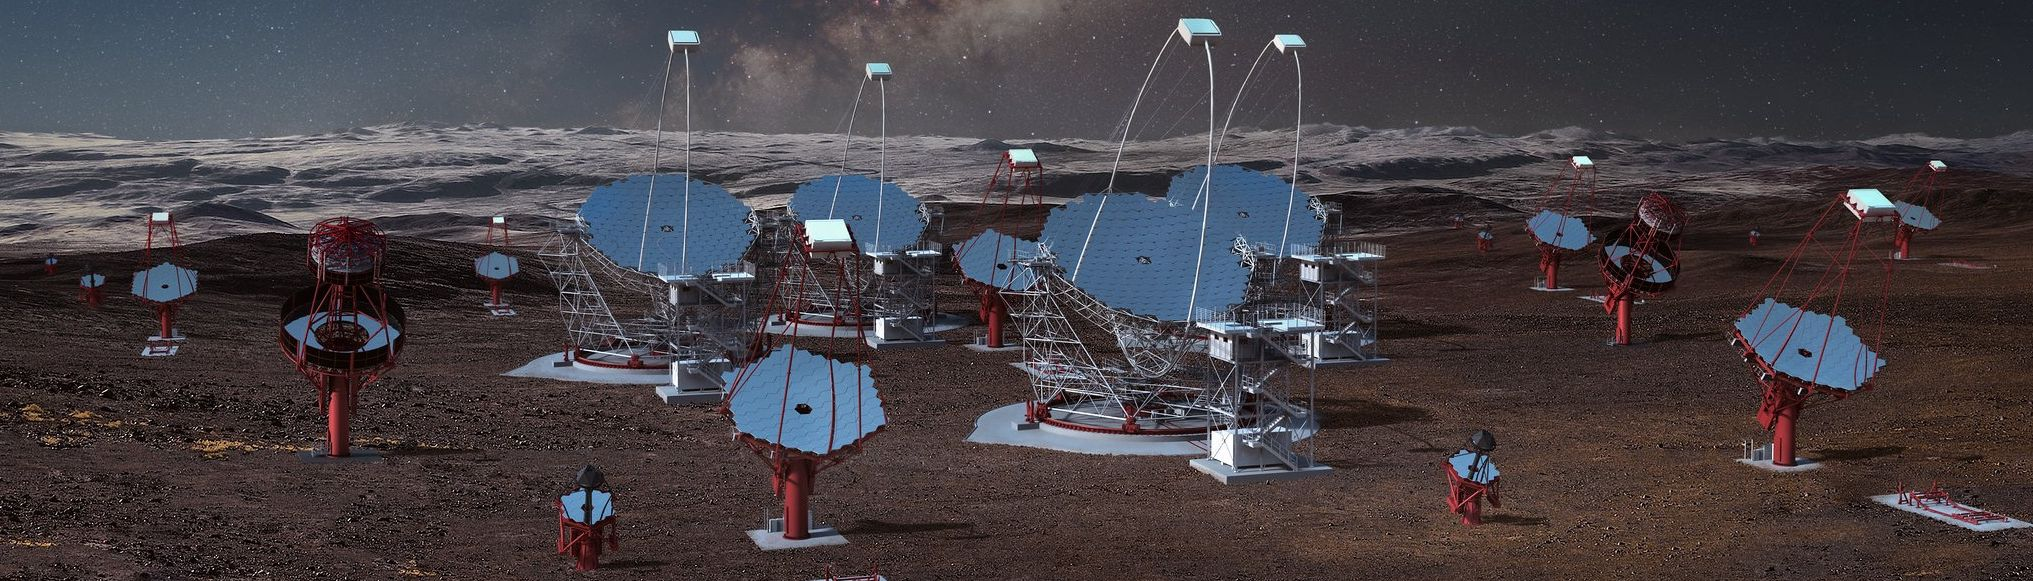
\includegraphics[width=\linewidth]{images/cta_south.jpg}
    \end{column}%
  \end{columns}
  \medskip

  \begin{center}
    \textasciitilde 30\,PB / year of archived raw data | High Level Reconstructed Data Published after Proprietary Period
  \end{center}
\end{frame}

\begin{frame}{ctapipe}
  \begin{itemize}
    \item Library and Tools for IACT event reconstruction
    \item Core library of the CTAO Data Processing and Preservation System (DPPS)
    \item Open, community-based development steered by CTAO maintainers
    \item \href{https://github.com/cta-observatory/ctapipe}{github.com/cta-observatory/ctapipe}
    \item Current release: \texttt{v0.18.1} – 2023-03-17
      \href{https://doi.org/10.5281/zenodo.3372210}{
\includegraphics[height=2ex]{images/ctapipe_zenodo.pdf}}
      \href{https://pypi.org/project/ctapipe}{
\includegraphics[height=2ex]{images/ctapipe_pypi.pdf}}
      \href{https://anaconda.org/conda-forge/ctapipe}{
\includegraphics[height=2ex]{images/ctapipe_conda.pdf}}
  \end{itemize}
\end{frame}

\begin{frame}
  \resizebox{\textwidth}{!}{%
\begin{tikzpicture}
  \tikzset{arrow/.style={-{Triangle Cap}, line width=10pt, shorten >= 5pt, shorten <= 5pt}}
  \tikzset{lightbg/.style={fill=lightgray, rounded corners=0.5cm, inner sep=0.2cm}}

  \node[] (ctapipe) at (0, 0) {
\includegraphics[width=10cm]{logos/ctapipe_logo_square.png}};

  \node[anchor=east, lightbg] (astropy) at (-8, 4.5) {
\includegraphics[height=2cm]{logos/astropy.pdf}};
  \node[anchor=north west, yshift=-0.5cm] (sklearn) at (astropy.south west) {
\includegraphics[height=2cm]{logos/sklearn.pdf}};
  \node[anchor=north west, yshift=-0.5cm] (numpy) at (sklearn.south west) {
\includegraphics[height=2cm]{logos/numpy.pdf}};
  \node[anchor=north west, yshift=-0.5cm, lightbg] (scipy) at (numpy.south west) {
\includegraphics[height=2cm]{logos/scipy.png}};
  \node[anchor=north west, yshift=-0.5cm] (pytables) at (scipy.south west) {
\includegraphics[height=2cm]{logos/pytables.png}};
  \node[anchor=north west, yshift=-0.5cm, lightbg] (matplotlib) at (pytables.south west) {
\includegraphics[height=2cm]{logos/matplotlib.pdf}};

  \draw[arrow, color=lightblue] (astropy.east) to[out=0, in=120] (120:5cm);
  \draw[arrow, color=lightblue] (sklearn.east) to[out=0, in=150] (150:5cm);
  \draw[arrow, color=lightblue] (numpy.east) to[out=0, in=170] (170:5cm);
  \draw[arrow, color=lightblue] (scipy.east) to[out=0, in=190] (190:5cm);
  \draw[arrow, color=lightblue] (pytables.east) to[out=0, in=200] (210:5cm);
  \draw[arrow, color=lightblue] (matplotlib.east) to[out=0, in=200] (230:5cm);

  \node[rectangle, fill=lightblue, minimum width=4.5cm, minimum height=4.5cm, text=white, anchor=north east, xshift=-0.25cm, yshift=-1cm, align=center, text width=4cm] (algos) at (ctapipe.south) {\Huge Algorithms\\\Huge \strut python, \strut numpy, \strut scipy};
  \node[rectangle, fill=darkblue, minimum width=4.5cm, minimum height=4.5cm, text=white, anchor=north west, xshift=0.25cm, yshift=-1cm, align=center] (numba) at (ctapipe.south) {\Huge Algorithms\\\Large Jit Compiled using \\ 
\includegraphics[width=4cm]{logos/numba.pdf}};

  \draw[{Triangle Cap}-{Triangle Cap}, color=darkblue, line width=10pt] (algos.north) to[out=90, in=245] (245:5cm);
  \draw[{Triangle Cap}-{Triangle Cap}, color=darkblue, line width=10pt] (numba.north) to[out=90, in=295] (295:5cm);

  \node[rectangle, fill=apps, minimum width=4.5cm, text width=4.5cm, minimum height=4.5cm, text=white, anchor=south west, yshift=0.25cm, xshift=1cm, align=center, font=\fontsize{32}{32}\selectfont] (tools) at (ctapipe.east) {pipeline\\tools};
  % \node[rectangle, fill=apps, minimum width=4.5cm, text width=4.5cm, minimum height=4.5cm, text=white, anchor=north west, yshift=-0.25cm, xshift=1cm, align=center, font=\huge] (advanced) at (ctapipe.east) {advanced\\pipeline\\applications};
  \node[anchor=north, yshift=-2.5cm, fill=apps] (jupyter) at (tools.south) {
\includegraphics[width=4cm]{logos/jupyter.pdf}};

  \draw[{Triangle Cap}-{Triangle Cap}, color=apps, line width=10pt] (tools.west) to[out=180, in=25] (25:5cm);
  % \draw[{Triangle Cap}-{Triangle Cap}, color=apps, line width=10pt] (advanced.west) to[out=180, in=-25] (-25:5cm);
  \draw[{Triangle Cap}-{Triangle Cap}, color=apps, line width=10pt] (jupyter.west) to[out=135, in=-45] (-45:5cm);

  \node[anchor=west, color=red!60!yellow, font=\Huge, yshift=1cm, xshift=0.5cm, text width=4cm] (deploy) at (tools.north east) {CI, Release \& Deploy};
  \node[anchor=north] (conda) at (deploy.south) {
\includegraphics[width=4cm]{logos/conda.pdf}};
  \node[anchor=north, yshift=-0.5cm] (forge) at (conda.south) {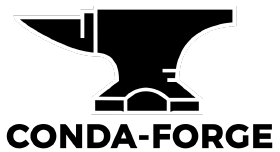
\includegraphics[width=4cm]{logos/conda-forge.png}};
  \node[anchor=north, yshift=-0.5cm] (pypi) at (forge.south) {
\includegraphics[width=4cm]{logos/pypi.pdf}};
  \node[anchor=north, yshift=-0.5cm] (pytest) at (pypi.south) {
\includegraphics[width=4cm]{logos/pytest.pdf}};
  \node[anchor=north, yshift=-0.5cm] (github) at (pytest.south) {
\includegraphics[width=4cm]{logos/github.pdf}};
\end{tikzpicture}
}

\end{frame}

\begin{frame}{Data Levels and Processing Steps}
  \vspace{-0.5cm}%
  \begin{tikzpicture}
  \tikzset{datalevel/.style={thick, circle, draw, inner sep=2pt, minimum size=25pt}}
  \tikzset{analysis-step/.style={align=center, font=\footnotesize}}
  \tikzset{step-arrow/.style={-{Triangle Cap}, line width=5pt, shorten >= 5pt, shorten <= 5pt}}

    % raw data plot
    \node[] (R0Graph)   at (0.0, 0) {\includegraphics[height=1.75cm]{build/r0.pdf}};
    \node[] (R1Graph)   at (2.5, 0) {\includegraphics[height=1.75cm]{build/r1.pdf}};
    \node[] (DL0Graph)  at (5.0, 0) {\includegraphics[height=1.75cm]{build/dl0.pdf}};

    \node[] (DL1ImageGraph)   at (10.0, 0.0) {\includegraphics[height=2.5cm]{build/dl1a.pdf}};
    \node[] (DL1CleanGraph) at (10.0, -5) {\includegraphics[height=2.5cm]{build/dl1a_clean.pdf}};

    % Param table
    \node [font=\scriptsize] (DL1bTable) at (1.5, -6) {
      \SetTblrInner{rowsep=0pt, colsep=2pt}
      \begin{tblr}{
          colspec={rrrrcr},
          row{1}={font=\bfseries},
      }
        event &  hillas\_intensity & hillas\_width  & hillas\_length  & $\cdots$ & concentration\_cog \\
          0 &  1253.1    &  0.15  &   0.52  & $\cdots$ & 0.35 \\
          2 &   321.3    &  0.05  &   0.12  & $\cdots$ & 0.42 \\
          5 &   512.7    &  0.08  &   0.19  & $\cdots$ & 0.45 \\
      \end{tblr}
    };

    % Reconstruction table
    \node[font=\scriptsize] (DL2Table) at (1, -3.5) {
        \SetTblrInner{rowsep=0pt, colsep=2pt}
        \begin{tblr}{
            colspec={rrrrrr},
            row{1}={font=\bfseries},
        }
        event & energy & gammaness &    ra &    dec &        time \\
              &        &           &   deg &    deg &        mjd  \\
            0 &   1500 &      0.82 &  83.6 &   22.1 & 59024.63123 \\
            2 &    400 &      0.73 &  83.5 &   21.9 & 59024.64183 \\
            5 &    680 &      0.92 &  83.7 &   22.0 & 59024.67093 \\
        \end{tblr}
    };

    \node [datalevel, color=gray, anchor=north]    (R0)   at (R0Graph.south)   {R0};
    \node [datalevel, color=gray, anchor=north]    (R1)   at (R1Graph.south)   {R1};
    \node [datalevel, anchor=north]                (DL0)  at (DL0Graph.south) {DL0};
    \node [datalevel, anchor=east, xshift=1.3cm, yshift=-0.1cm] (DL1Image) at (DL1ImageGraph.south west) {DL1a};
    \node [datalevel, anchor=east, xshift=0.7cm, yshift=-0.1cm] (DL1Clean) at (DL1CleanGraph.north west) {DL1a};
    \node [datalevel, anchor=west] (DL1b) at (DL1bTable.east) {DL1b};
    \node [datalevel, anchor=west] (DL2)  at (DL2Table.east) {DL2};

    \draw[step-arrow, color=gray] (R0.east) -- (R1.west)  node [analysis-step, midway, below, text width=2cm] {Low-Level\\Calibration};
    \draw[step-arrow, color=gray] (R1.east) -- (DL0.west)  node [analysis-step, midway, below, text width=2cm] {Data Volume\\ Reduction};
    \draw[step-arrow] (DL0.east) -- (DL1Image.west)  node [analysis-step, midway, below, yshift=-0.15cm] {Pulse Extraction};
    \draw[step-arrow] (DL1Image.south east) to[out=315, in=45]  node [analysis-step, midway, right, xshift=0.2cm] {Image Cleaning} (DL1Clean.north east); 
    \draw[step-arrow] (DL1Clean.south) to[bend left] node [analysis-step, midway, above, xshift=-0.7cm, yshift=0.3cm] {Parametrization} (DL1b.east);
    \draw[step-arrow] (DL1b.110) -- (DL2.south east)  node [analysis-step, midway, left, yshift=-0.2cm] {Reconstruction};

\end{tikzpicture}

\end{frame}

\begin{frame}{Release 0.18(.1)}
  \begin{itemize}
    \item New reconstruction methods based on sklearn
      \begin{itemize}
        \item Particle Classification (Gamma / Hadron)
        \item Primary Energy
        \item Disp-Method for direction reconstruction
      \end{itemize}
    \item CLI-Applications to train / apply models
    \item Plugin system also for reconstruction methods
  \end{itemize}

  \bigskip
  \begin{center}
    \large
    $\Rightarrow$ ctapipe now able to produce fully reconstructed DL2 event data
  \end{center}
\end{frame}

\begin{frame}{Data Format}
  \begin{columns}[c, onlytextwidth]
    \begin{column}{0.4\textwidth}
      \begin{itemize}
        \item Plugin-System for input data
        \item HDF5 for output, including rich metadata, compression, transformations
        \item Utilities for bulk loading data into  \texttt{astropy.table.Table}s
      \end{itemize}
    \end{column}%
    \hfill%
    \begin{column}{0.59\textwidth}%
      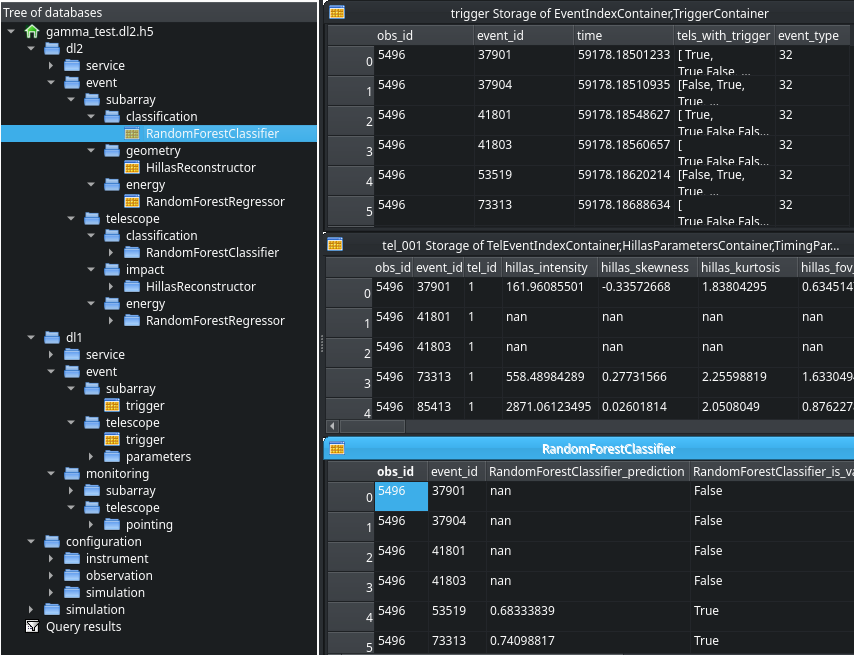
\includegraphics[width=\linewidth]{./images/ctapipe_hdf5.png}
    \end{column}%
  \end{columns}
\end{frame}


\begin{frame}{Public DL1 / DL2 Data Release}
  \begin{itemize}
    \item Newly released dataset on Zenodo
    \item Simulated gamma-ray and proton events at DL1 (including images) and DL2 (only geometry) 
    \item 50 GB (size limit of Zenodo)
    \item ca.~ 500\,000 successfully reconstructed array events for each particle type
    \item Well-suited for machine learning studies at all levels
    \item Public, cite-able dataset: \href{https://doi.org/10.5281/zenodo.7298568}{
\includegraphics[height=2ex]{./images/public_data_zenodo.pdf}}

    \item Everything shown in the following uses this dataset, full workflow / talk source available here: \\
      \href{https://github.com/maxnoe/ctapipe-dpg-2023}{github.com/maxnoe/ctapipe-dpg-2023}
  \end{itemize}
\end{frame}

\begin{frame}{New Machine Learning Reconstruction}
  \begin{itemize}
    \item Based on scikit-learn
    \item Very flexible thanks to integration with the ctapipe
    \item Procedure (as of 0.18.0):
      \begin{itemize}
        \item Training of models per telescope type
        \item Weighted average of telescope-wise predictions for final array event prediction\\
          See Lukas Beiske's talk for a nested model approach (AKPIK 2.8) 
      \end{itemize}
    \item Models for
      \begin{itemize}
        \item Energy (1D Regression)
        \item Particle Classification (Binary Classification)
        \item Direction reconstruction using the disp method (1D Regression + Binary Classification)
      \end{itemize}
  \end{itemize}
\end{frame}

\begin{frame}{Standard Workflow DL0 → DL2}
  \begin{tikzpicture}
  \newcommand\file[1]{\faIcon{file}\,\texttt{#1}}
  \tikzset{arrow/.style={-{Triangle Cap}, line width=3pt, shorten >= 2pt, shorten <= 2pt}}
  \tikzset{tool/.style={color=tugreen, font=\ttfamily}}

  \node[anchor=north west] (gamma1) at (0, 0) {\file{sim. run 1}};
  \node[anchor=north west] (gamma2) at (gamma1.south west) {\file{sim. run 2}};
  \node[anchor=north west] (gamma3) at (gamma2.south west) {\file{sim. run 3}};

  \node[anchor=west, xshift=0.5cm, tool] (process1) at (gamma1.east) {process};
  \node[anchor=west, xshift=0.5cm, tool] (process2) at (gamma2.east) {process};
  \node[anchor=west, xshift=0.5cm, tool] (process3) at (gamma3.east) {process};

  \node[anchor=west, xshift=0.5cm] (gamma-dl1-1) at (process1.east) {\file{run 1 dl1/dl2}};
  \node[anchor=west, xshift=0.5cm] (gamma-dl1-2) at (process2.east) {\file{run 2 dl1/dl2}};
  \node[anchor=west, xshift=0.5cm] (gamma-dl1-3) at (process3.east) {\file{run 3 dl1/dl2}};

  \draw[arrow] (gamma1.east) to (process1.west);
  \draw[arrow] (gamma2.east) to (process2.west);
  \draw[arrow] (gamma3.east) to (process3.west);
  \draw[arrow] (process1.east) to (gamma-dl1-1.west);
  \draw[arrow] (process2.east) to (gamma-dl1-2.west);
  \draw[arrow] (process3.east) to (gamma-dl1-3.west);

  \node[anchor=west, xshift=0.5cm, tool] (merge1) at (gamma-dl1-2.east) {merge};
  \node[anchor=west, xshift=0.5cm] (merge1-out) at (merge1.east) {\file{merged dl1/dl2 dataset}};

  \draw[arrow] (gamma-dl1-1.east) to[bend left] (merge1.west);
  \draw[arrow] (gamma-dl1-2.east) to (merge1.west);
  \draw[arrow] (gamma-dl1-3.east) to[bend right] (merge1.west);
  \draw[arrow] (merge1.east) to (merge1-out.west);
\end{tikzpicture}



  \bigskip
  \begin{itemize}
    \item Process many simulation runs in parallel to DL1 plus DL2 geometry
    \item Merge into large datasets
    \item DL1 step also includes selection of a specific CTAO array from the simulated super-array
  \end{itemize}
\end{frame}
\begin{frame}{Standard Workflow DL0 → DL2}
  \vspace{0.5cm}
\begin{tikzpicture}
  \newcommand\file[1]{\faIcon{file}\,\texttt{#1}}
  \tikzset{arrow/.style={-{Triangle Cap}, line width=3pt, shorten >= 2pt, shorten <= 2pt}}
  \tikzset{tool/.style={color=tugreen, font=\ttfamily}}



  \node[anchor=north west, text width=3cm] (gamma-train-en) at (0, 0) {\file{gamma-train-en}};
  \node[anchor=west, xshift=0.5cm, tool] (train-energy) at (gamma-train-en.east) {train-energy-regressor};
  \node[anchor=north, yshift=-0.5cm] (energy-model) at (train-energy.south) {\file{energy model}};
  \node[anchor=west, xshift=0.5cm, tool] (train-energy) at (gamma-train-en.east) {train-energy-regressor};

  \node[anchor=north, yshift=-0.5cm, tool] (apply-gamma-train) at (energy-model.south) {apply-models};
  \node[anchor=east, text width=3cm, xshift=-0.5cm] (gamma-train-clf) at (apply-gamma-train.west) {\file{gamma-train-clf}};
  \node[anchor=west, xshift=0.5cm] (gamma-train-clf-tmp) at (apply-gamma-train.east) {\file{}};

  \node[anchor=north west, text width=3cm] (proton-train-clf) at (gamma-train-clf.south west) {\file{proton-train-clf}};

  \node[anchor=west, xshift=0.5cm, tool] (apply-proton-train) at (proton-train-clf.east) {apply-models};
  \node[anchor=west, xshift=0.5cm] (proton-train-clf-tmp) at (apply-proton-train.east) {\file{}};


  \draw[arrow] (gamma-train-en.east) to (train-energy.west);
  \draw[arrow] (train-energy.south) to (energy-model.north);


  \draw[arrow] (energy-model.south) to (apply-gamma-train.north);
  \draw[arrow] (apply-gamma-train.east) to (gamma-train-clf-tmp.west);
  \draw[arrow] (gamma-train-clf.east) to (apply-gamma-train.west);
  \draw[arrow] (apply-proton-train.east) to (proton-train-clf-tmp.west);
  \draw[arrow] (proton-train-clf.east) to (apply-proton-train.west);

  \node[anchor=west, xshift=0.5cm, tool] (train-classifier) at (gamma-train-clf-tmp.south east) {train-particle-classifier};
  \draw[arrow] (gamma-train-clf-tmp.east) to[bend left] (train-classifier.west);
  \draw[arrow] (proton-train-clf-tmp.east) to[bend right] (train-classifier.west);

  \node[anchor=north, yshift=-0.5cm] (classifier) at (train-classifier.south) {\file{particle classification model}};
  \draw[arrow] (train-classifier.south) to (classifier.north);

  \node[anchor=north, yshift=-0.5cm, tool] (apply-gamma-eval) at (classifier.south) {apply-models};
  \draw[arrow] (classifier.south) to (apply-gamma-eval.north);

  \node[anchor=east, text width=2.5cm, xshift=-0.5cm] (gamma-eval) at (apply-gamma-eval.west) {\file{gamma-eval}};
  \draw[arrow] (gamma-eval.east) to (apply-gamma-eval.west);

  \node[anchor=north west, text width=2.5cm] (proton-eval) at (gamma-eval.south west) {\file{proton-eval}};
  \node[anchor=west, xshift=0.5cm, tool] (apply-proton-eval) at (proton-eval.east) {apply-models};
  \draw[arrow] (proton-eval.east) to (apply-proton-eval.west);

  % \node[anchor=north west, text width=2.5cm] (electron-eval) at (proton-eval.south west) {\file{electron-eval}};
  % \node[anchor=west, xshift=0.5cm, tool] (apply-electron-eval) at (electron-eval.east) {apply-models};
  % \draw[arrow] (electron-eval.east) to (apply-electron-eval.west);

  \node[anchor=west, xshift=0.5cm] (gamma-final) at (apply-gamma-eval.east) {\file{gamma-eval}};
  \draw[arrow] (apply-gamma-eval) to (gamma-final);

  \node[anchor=west, xshift=0.5cm] (proton-final) at (apply-proton-eval.east) {\file{proton-eval}};
  \draw[arrow] (apply-proton-eval) to (proton-final);

  \node[anchor=north, yshift=-0.5cm] (energy-model) at (apply-proton-eval.south) {\file{energy model}};
  \draw[arrow] (energy-model) to (apply-proton-eval);

  % \node[anchor=west, xshift=0.5cm] (electron-final) at (apply-electron-eval.east) {\file{electron eval}};
  % \draw[arrow] (apply-electron-eval) to (electron-final);

\end{tikzpicture}

\end{frame}

\begin{frame}{Example yaml configuration}
  \footnotesize
  \begin{columns}[t, onlytextwidth]
    \begin{column}{0.495\textwidth}
      \inputminted[firstline=8, lastline=30]{yaml}{./config/train_energy_regressor.yml}
    \end{column}%
    \hfill%
    \begin{column}{0.495\textwidth}%
      \inputminted[firstline=31, lastline=50]{yaml}{./config/train_energy_regressor.yml}
      \hspace{4em}\texttt{...}
    \end{column}%
  \end{columns}
\end{frame}

\begin{frame}[c]
  \centering
  % \begin{columns}[c, onlytextwidth]
  %   \begin{column}{0.7\textwidth}
  %     \only<1>{%
        \includegraphics{./build/plots/energy_migration.pdf}
      % }%
      % \only<2>{%
      %   \includegraphics{./build/plots/energy_migration_gammaness.pdf}
      % }%
    % \end{column}%
    % \hfill%
    % \begin{column}{0.295\textwidth}%
    %   % Energy Migration\\
    %   % \onslide<2>{for \texttt{gammaness} > 0.5}
    % \end{column}
  % \end{columns}
\end{frame}

% \begin{frame}[c]
%   \centering
%   \includegraphics{./build/plots/gammaness_energy.pdf}
% \end{frame}

\begin{frame}[c]
  \centering
  \includegraphics{./build/plots/roc.pdf}
\end{frame}

\begin{frame}{Conclusion and Future Plans}
  \begin{itemize}
    \item With ctapipe 0.18, fully reconstructed DL2 events possible
    \item Classical machine learning using sklearn
    \item Plugin system for other reconstrucion methods (deep learning, likelihood, etc.)
    \item Public data release on Zenodo
    \item New proposal process for large changes to ctapipe
    \item Next steps
      \begin{itemize}
        \item Computation of Instrument Response Functions (using pyirf)
        \item Categorization of events into different event types
        \item Towards analysis of observed data: monitoring / calibration / service
      \end{itemize}
  \end{itemize}
\end{frame}

\end{document}
